\documentclass[9pt,hyperref={pdfpagemode=FullScreen,urlcolor=blue},xcolor=x11names]{beamer}

\mode<presentation>
{
  \usetheme{Warsaw}
  %\usetheme{Darmstadt}
  %\usetheme{Marburg}
  \setbeamertemplate{navigation symbols}{}

  %\usecolortheme{crane}
  %\usecolortheme{rose,sidebartab}

  \usecolortheme{beaver}
  %\usecolortheme{lily,sidebartab}
  %\usecolortheme{seahorse}

  \usefonttheme{serif}

  \setbeamertemplate{footline}[page number]
  \setbeamertemplate{sidebar canvas right}[vertical shading][top=palette
  primary.bg,%,middle=white,
  bottom=palette primary.bg]
  %\setbeamertemplate{sections/subsections in toc}[section numbered,subsection numbered]

  %\setbeamertemplate{itemize subitem}[circle]

  \setbeamercovered{transparent}

  %\beamertemplatenavigationsymbolsempty

  \useinnertheme{default}
}

\usepackage[utf8]{inputenc}
\usepackage[T1]{fontenc}
\usepackage{lmodern}
\usepackage{xspace}
\usepackage{amsmath,amssymb}
\usepackage[english]{babel}
%\usepackage[latin1]{inputenc}
%\usepackage[T1]{fontenc}
\usepackage{aeguill,fourier}

% souligne, barre
\usepackage{ulem}
%\usepackage[x11names]{xcolor}

\usepackage{pgf,pgfarrows,pgfnodes,pgfautomata,pgfheaps,pgfshade}

\usepackage{wasysym}
\usepackage{fancyvrb}
%\usepackage{verbatim}
%\usepackage{marvosym}
\usepackage{eurosym} % symbol euro

\usepackage{colortbl}

\usepackage{pdftricks}
\begin{psinputs}
\usepackage{pstricks}
\usepackage{pst-bar}
\usepackage{pstricks-add}
\end{psinputs}

\usepackage{ulem}

\usepackage{ifdraft}
\usepackage{animate}
\usepackage{multimedia}

%\usepackage{texmath}

\usepackage{tikz}
\usetikzlibrary{calc}
\usetikzlibrary{patterns}   % for hatching
\usetikzlibrary{positioning}
\usetikzlibrary{decorations.pathreplacing}
\usetikzlibrary{decorations.pathmorphing}
\usetikzlibrary{arrows, decorations.markings}
\usetikzlibrary{shapes.geometric}
\newcommand{\warningsign}{\tikz[baseline=-.75ex] \node[shape=regular polygon, regular polygon sides=3, inner sep=0pt, draw, thick] {\textbf{!}};}
\newcommand{\reddanger}{\textcolor{red}{\danger}}


% the following is from 
% http://tex.stackexchange.com/questions/4811/make-first-row-of-table-all-bold
%\usepackage{array}
%\newcolumntype{$}{>{\global\let\currentrowstyle\relax}}
%\newcolumntype{^}{>{\currentrowstyle}}
%\newcommand{\rowstyle}[1]{\gdef\currentrowstyle{#1}%
%  #1\ignorespaces
%}

\usepackage{listings}
\usepackage{minted}

\usepackage{caption}


%%%%%%%%%%%%%%%%%%%
\hypersetup{%
  pdftitle={PATC-KOKKOS-2018},%
  pdfauthor={Pierre Kestener - CEA Saclay - MDLS - http://www.maisondelasimulation.fr},
  pdfsubject={Introdcution to Kokkos},
  pdfkeywords={KOKKOS, C++, GPU},
  pdfproducer={pdflatex avec la classe BEAMER},
  bookmarksopen=false,
  urlcolor=blue
}

%%%%%%%%%%%%%%%%%%%%%%%%%%%%%%%%%%%%%%%%%%%%%%%%%%%%%%%%%%%%%%%
%%%%%%%%%%%%%%%%%%%%%%%%%%%%%%%%%%%%%%%%%%%%%%%%%%%%%%%%%%%%%%%
%%%%%%%%%%%%%%%%%%%%%%%%%%%%%%%%%%%%%%%%%%%%%%%%%%%%%%%%%%%%%%%

%\title{Kokkos, Modern C++, performance portability, ...}
\title{Introduction to performance portability. Mini-overview of Kokkos/C++ library.}

\author
{
  \mbox{\underline{Pierre Kestener}}\inst{1}
}

\institute[mdls sap]{%
  \inst{1}%
  CEA Saclay, DRF, Maison de la Simulation
}

\date{PATC, April 1st - April 2nd, 2018}

\pgfdeclareimage[height=0.5cm]{university-logo}{./images/Sigle-mdls}
\logo{\pgfuseimage{university-logo}}


%%%%%%%%%%%%%%%%%%%%%
\pgfdeclareimage[width=2.0cm]{sigle-cea}{./images/Sigle-mdls}
\pgfdeclareimage[width=2.0cm]{sigle-prace}{images/logo_prace}
\pgfdeclareimage[width=2.0cm]{sigle-nvidia}{images/NV_CUDA_Teaching_Center_3D.jpg}

\titlegraphic{
  % \pgfuseimage{sigle-prace}
  \hfill
  \pgfuseimage{sigle-cea}
  \hfill
  % \pgfuseimage{sigle-nvidia}
}



\begin{document}


\definecolor{green2}{rgb}{0.1,0.8,0.1} 
\definecolor{trust}{rgb}{0.71,0.14,0.07}
\definecolor{FancyPurple}{rgb}{0.5176, 0.1137, 0.2314}

\colorlet{redshaded}{red!25!bg}
\colorlet{shaded}{black!25!bg}
\colorlet{shadedshaded}{black!10!bg}
\colorlet{blackshaded}{black!40!bg}

\colorlet{darkred}{red!80!black}
\colorlet{darkblue}{blue!80!black}
\colorlet{darkgreen}{green!70!black}
\colorlet{greenshaded}{green!95!bg}
%\colorlet{coral}{Coral1!95!bg}

%red, green, blue, cyan, magenta, yellow, black, white, darkgray, gray,
%lightgray, brown, lime, olive, orange, pink, purple, teal, violet

\newcommand\myurl[1]{\textcolor{purple}{\underline{\url{#1}}}}
\newcommand\myhref[2]{\textcolor{purple}{\underline{\href{#1}{#2}}}}

\newcommand\mySmiley{\textcolor{darkgreen}{\Smiley{}}}
\newcommand\myFrowny{\textcolor{red}{\Frowny{}}}

%% Big-O notation.
\providecommand{\OO}[1]{\ensuremath{\operatorname{O}\bigl(#1\bigr)}}

% definition des couleurs pour affichage de code
\makeatletter
\def\PY@reset{\let\PY@it=\relax \let\PY@bf=\relax%
    \let\PY@ul=\relax \let\PY@tc=\relax%
    \let\PY@bc=\relax \let\PY@ff=\relax}
\def\PY@tok#1{\csname PY@tok@#1\endcsname}
\def\PY@toks#1+{\ifx\relax#1\empty\else%
    \PY@tok{#1}\expandafter\PY@toks\fi}
\def\PY@do#1{\PY@bc{\PY@tc{\PY@ul{%
    \PY@it{\PY@bf{\PY@ff{#1}}}}}}}
\def\PY#1#2{\PY@reset\PY@toks#1+\relax+\PY@do{#2}}

\def\PY@tok@gd{\def\PY@tc##1{\textcolor[rgb]{0.63,0.00,0.00}{##1}}}
\def\PY@tok@gu{\let\PY@bf=\textbf\def\PY@tc##1{\textcolor[rgb]{0.50,0.00,0.50}{##1}}}
\def\PY@tok@gt{\def\PY@tc##1{\textcolor[rgb]{0.00,0.25,0.82}{##1}}}
\def\PY@tok@gs{\let\PY@bf=\textbf}
\def\PY@tok@gr{\def\PY@tc##1{\textcolor[rgb]{1.00,0.00,0.00}{##1}}}
\def\PY@tok@cm{\let\PY@it=\textit\def\PY@tc##1{\textcolor[rgb]{0.25,0.50,0.50}{##1}}}
\def\PY@tok@vg{\def\PY@tc##1{\textcolor[rgb]{0.10,0.09,0.49}{##1}}}
\def\PY@tok@m{\def\PY@tc##1{\textcolor[rgb]{0.40,0.40,0.40}{##1}}}
\def\PY@tok@mh{\def\PY@tc##1{\textcolor[rgb]{0.40,0.40,0.40}{##1}}}
\def\PY@tok@go{\def\PY@tc##1{\textcolor[rgb]{0.50,0.50,0.50}{##1}}}
\def\PY@tok@ge{\let\PY@it=\textit}
\def\PY@tok@vc{\def\PY@tc##1{\textcolor[rgb]{0.10,0.09,0.49}{##1}}}
\def\PY@tok@il{\def\PY@tc##1{\textcolor[rgb]{0.40,0.40,0.40}{##1}}}
\def\PY@tok@cs{\let\PY@it=\textit\def\PY@tc##1{\textcolor[rgb]{0.25,0.50,0.50}{##1}}}
\def\PY@tok@cp{\def\PY@tc##1{\textcolor[rgb]{0.74,0.48,0.00}{##1}}}
\def\PY@tok@gi{\def\PY@tc##1{\textcolor[rgb]{0.00,0.63,0.00}{##1}}}
\def\PY@tok@gh{\let\PY@bf=\textbf\def\PY@tc##1{\textcolor[rgb]{0.00,0.00,0.50}{##1}}}
\def\PY@tok@ni{\let\PY@bf=\textbf\def\PY@tc##1{\textcolor[rgb]{0.60,0.60,0.60}{##1}}}
\def\PY@tok@nl{\def\PY@tc##1{\textcolor[rgb]{0.63,0.63,0.00}{##1}}}
\def\PY@tok@nn{\let\PY@bf=\textbf\def\PY@tc##1{\textcolor[rgb]{0.00,0.00,1.00}{##1}}}
\def\PY@tok@no{\def\PY@tc##1{\textcolor[rgb]{0.53,0.00,0.00}{##1}}}
\def\PY@tok@na{\def\PY@tc##1{\textcolor[rgb]{0.49,0.56,0.16}{##1}}}
\def\PY@tok@nb{\def\PY@tc##1{\textcolor[rgb]{0.00,0.50,0.00}{##1}}}
\def\PY@tok@nc{\let\PY@bf=\textbf\def\PY@tc##1{\textcolor[rgb]{0.00,0.00,1.00}{##1}}}
\def\PY@tok@nd{\def\PY@tc##1{\textcolor[rgb]{0.67,0.13,1.00}{##1}}}
\def\PY@tok@ne{\let\PY@bf=\textbf\def\PY@tc##1{\textcolor[rgb]{0.82,0.25,0.23}{##1}}}
\def\PY@tok@nf{\def\PY@tc##1{\textcolor[rgb]{0.00,0.00,1.00}{##1}}}
\def\PY@tok@si{\let\PY@bf=\textbf\def\PY@tc##1{\textcolor[rgb]{0.73,0.40,0.53}{##1}}}
\def\PY@tok@s2{\def\PY@tc##1{\textcolor[rgb]{0.73,0.13,0.13}{##1}}}
\def\PY@tok@vi{\def\PY@tc##1{\textcolor[rgb]{0.10,0.09,0.49}{##1}}}
\def\PY@tok@nt{\let\PY@bf=\textbf\def\PY@tc##1{\textcolor[rgb]{0.00,0.50,0.00}{##1}}}
\def\PY@tok@nv{\def\PY@tc##1{\textcolor[rgb]{0.10,0.09,0.49}{##1}}}
\def\PY@tok@s1{\def\PY@tc##1{\textcolor[rgb]{0.73,0.13,0.13}{##1}}}
\def\PY@tok@sh{\def\PY@tc##1{\textcolor[rgb]{0.73,0.13,0.13}{##1}}}
\def\PY@tok@sc{\def\PY@tc##1{\textcolor[rgb]{0.73,0.13,0.13}{##1}}}
\def\PY@tok@sx{\def\PY@tc##1{\textcolor[rgb]{0.00,0.50,0.00}{##1}}}
\def\PY@tok@bp{\def\PY@tc##1{\textcolor[rgb]{0.00,0.50,0.00}{##1}}}
\def\PY@tok@c1{\let\PY@it=\textit\def\PY@tc##1{\textcolor[rgb]{0.25,0.50,0.50}{##1}}}
\def\PY@tok@kc{\let\PY@bf=\textbf\def\PY@tc##1{\textcolor[rgb]{0.00,0.50,0.00}{##1}}}
\def\PY@tok@c{\let\PY@it=\textit\def\PY@tc##1{\textcolor[rgb]{0.25,0.50,0.50}{##1}}}
\def\PY@tok@mf{\def\PY@tc##1{\textcolor[rgb]{0.40,0.40,0.40}{##1}}}
\def\PY@tok@err{\def\PY@bc##1{\fcolorbox[rgb]{1.00,0.00,0.00}{1,1,1}{##1}}}
\def\PY@tok@kd{\let\PY@bf=\textbf\def\PY@tc##1{\textcolor[rgb]{0.00,0.50,0.00}{##1}}}
\def\PY@tok@ss{\def\PY@tc##1{\textcolor[rgb]{0.10,0.09,0.49}{##1}}}
\def\PY@tok@sr{\def\PY@tc##1{\textcolor[rgb]{0.73,0.40,0.53}{##1}}}
\def\PY@tok@mo{\def\PY@tc##1{\textcolor[rgb]{0.40,0.40,0.40}{##1}}}
\def\PY@tok@kn{\let\PY@bf=\textbf\def\PY@tc##1{\textcolor[rgb]{0.00,0.50,0.00}{##1}}}
\def\PY@tok@mi{\def\PY@tc##1{\textcolor[rgb]{0.40,0.40,0.40}{##1}}}
\def\PY@tok@gp{\let\PY@bf=\textbf\def\PY@tc##1{\textcolor[rgb]{0.00,0.00,0.50}{##1}}}
\def\PY@tok@o{\def\PY@tc##1{\textcolor[rgb]{0.40,0.40,0.40}{##1}}}
\def\PY@tok@kr{\let\PY@bf=\textbf\def\PY@tc##1{\textcolor[rgb]{0.00,0.50,0.00}{##1}}}
\def\PY@tok@s{\def\PY@tc##1{\textcolor[rgb]{0.73,0.13,0.13}{##1}}}
\def\PY@tok@kp{\def\PY@tc##1{\textcolor[rgb]{0.00,0.50,0.00}{##1}}}
\def\PY@tok@w{\def\PY@tc##1{\textcolor[rgb]{0.73,0.73,0.73}{##1}}}
\def\PY@tok@kt{\def\PY@tc##1{\textcolor[rgb]{0.69,0.00,0.25}{##1}}}
\def\PY@tok@ow{\let\PY@bf=\textbf\def\PY@tc##1{\textcolor[rgb]{0.67,0.13,1.00}{##1}}}
\def\PY@tok@sb{\def\PY@tc##1{\textcolor[rgb]{0.73,0.13,0.13}{##1}}}
\def\PY@tok@k{\let\PY@bf=\textbf\def\PY@tc##1{\textcolor[rgb]{0.00,0.50,0.00}{##1}}}
\def\PY@tok@se{\let\PY@bf=\textbf\def\PY@tc##1{\textcolor[rgb]{0.73,0.40,0.13}{##1}}}
\def\PY@tok@sd{\let\PY@it=\textit\def\PY@tc##1{\textcolor[rgb]{0.73,0.13,0.13}{##1}}}

\def\PYZbs{\char`\\}
\def\PYZus{\char`\_}
\def\PYZob{\char`\{}
\def\PYZcb{\char`\}}
\def\PYZca{\char`\^}
\def\PYZsh{\char`\#}
\def\PYZpc{\char`\%}
\def\PYZdl{\char`\$}
\def\PYZti{\char`\~}

\newcommand\lb{[}
\newcommand\rb{]}
\newcommand\PYbg[1]{\textcolor[rgb]{0.00,0.50,0.00}{\textbf{#1}}}
\newcommand\PYbf[1]{\textcolor[rgb]{0.73,0.40,0.53}{\textbf{#1}}}
\newcommand\PYbe[1]{\textcolor[rgb]{0.40,0.40,0.40}{#1}}
\newcommand\PYbd[1]{\textcolor[rgb]{0.73,0.13,0.13}{#1}}
\newcommand\PYbc[1]{\textcolor[rgb]{0.00,0.50,0.00}{\textbf{#1}}}
\newcommand\PYbb[1]{\textcolor[rgb]{0.40,0.40,0.40}{#1}}
\newcommand\PYba[1]{\textcolor[rgb]{0.00,0.00,0.50}{\textbf{#1}}}
\newcommand\PYaJ[1]{\textcolor[rgb]{0.73,0.13,0.13}{#1}}
\newcommand\PYaK[1]{\textcolor[rgb]{0.00,0.00,1.00}{#1}}
\newcommand\PYaH[1]{\fcolorbox[rgb]{1.00,0.00,0.00}{1,1,1}{#1}}
\newcommand\PYaI[1]{\textcolor[rgb]{0.69,0.00,0.25}{#1}}
\newcommand\PYaN[1]{\textcolor[rgb]{0.00,0.00,1.00}{\textbf{#1}}}
\newcommand\PYaO[1]{\textcolor[rgb]{0.00,0.00,0.50}{\textbf{#1}}}
\newcommand\PYaL[1]{\textcolor[rgb]{0.73,0.73,0.73}{#1}}
\newcommand\PYaM[1]{\textcolor[rgb]{0.74,0.48,0.00}{#1}}
\newcommand\PYaB[1]{\textcolor[rgb]{0.00,0.25,0.82}{#1}}
\newcommand\PYaC[1]{\textcolor[rgb]{0.67,0.13,1.00}{#1}}
\newcommand\PYaA[1]{\textcolor[rgb]{0.00,0.50,0.00}{#1}}
\newcommand\PYaF[1]{\textcolor[rgb]{1.00,0.00,0.00}{#1}}
\newcommand\PYaG[1]{\textcolor[rgb]{0.10,0.09,0.49}{#1}}
\newcommand\PYaD[1]{\textcolor[rgb]{0.25,0.50,0.50}{\textit{#1}}}
\newcommand\PYaE[1]{\textcolor[rgb]{0.63,0.00,0.00}{#1}}
\newcommand\PYaZ[1]{\textcolor[rgb]{0.00,0.50,0.00}{\textbf{#1}}}
\newcommand\PYaX[1]{\textcolor[rgb]{0.00,0.50,0.00}{#1}}
\newcommand\PYaY[1]{\textcolor[rgb]{0.73,0.13,0.13}{#1}}
\newcommand\PYaR[1]{\textcolor[rgb]{0.10,0.09,0.49}{#1}}
\newcommand\PYaS[1]{\textcolor[rgb]{0.25,0.50,0.50}{\textit{#1}}}
\newcommand\PYaP[1]{\textcolor[rgb]{0.49,0.56,0.16}{#1}}
\newcommand\PYaQ[1]{\textcolor[rgb]{0.40,0.40,0.40}{#1}}
\newcommand\PYaV[1]{\textcolor[rgb]{0.00,0.00,1.00}{\textbf{#1}}}
\newcommand\PYaW[1]{\textcolor[rgb]{0.73,0.13,0.13}{#1}}
\newcommand\PYaT[1]{\textcolor[rgb]{0.50,0.00,0.50}{\textbf{#1}}}
\newcommand\PYaU[1]{\textcolor[rgb]{0.82,0.25,0.23}{\textbf{#1}}}
\newcommand\PYaj[1]{\textcolor[rgb]{0.00,0.50,0.00}{#1}}
\newcommand\PYak[1]{\textcolor[rgb]{0.73,0.40,0.53}{#1}}
\newcommand\PYah[1]{\textcolor[rgb]{0.63,0.63,0.00}{#1}}
\newcommand\PYai[1]{\textcolor[rgb]{0.10,0.09,0.49}{#1}}
\newcommand\PYan[1]{\textcolor[rgb]{0.67,0.13,1.00}{\textbf{#1}}}
\newcommand\PYao[1]{\textcolor[rgb]{0.73,0.40,0.13}{\textbf{#1}}}
\newcommand\PYal[1]{\textcolor[rgb]{0.25,0.50,0.50}{\textit{#1}}}
\newcommand\PYam[1]{\textbf{#1}}
\newcommand\PYab[1]{\textit{#1}}
\newcommand\PYac[1]{\textcolor[rgb]{0.73,0.13,0.13}{#1}}
\newcommand\PYaa[1]{\textcolor[rgb]{0.50,0.50,0.50}{#1}}
\newcommand\PYaf[1]{\textcolor[rgb]{0.25,0.50,0.50}{\textit{#1}}}
\newcommand\PYag[1]{\textcolor[rgb]{0.40,0.40,0.40}{#1}}
\newcommand\PYad[1]{\textcolor[rgb]{0.73,0.13,0.13}{#1}}
\newcommand\PYae[1]{\textcolor[rgb]{0.40,0.40,0.40}{#1}}
\newcommand\PYaz[1]{\textcolor[rgb]{0.00,0.63,0.00}{#1}}
\newcommand\PYax[1]{\textcolor[rgb]{0.60,0.60,0.60}{\textbf{#1}}}
\newcommand\PYay[1]{\textcolor[rgb]{0.00,0.50,0.00}{\textbf{#1}}}
\newcommand\PYar[1]{\textcolor[rgb]{0.10,0.09,0.49}{#1}}
\newcommand\PYas[1]{\textcolor[rgb]{0.73,0.13,0.13}{\textit{#1}}}
\newcommand\PYap[1]{\textcolor[rgb]{0.00,0.50,0.00}{#1}}
\newcommand\PYaq[1]{\textcolor[rgb]{0.53,0.00,0.00}{#1}}
\newcommand\PYav[1]{\textcolor[rgb]{0.00,0.50,0.00}{\textbf{#1}}}
\newcommand\PYaw[1]{\textcolor[rgb]{0.40,0.40,0.40}{#1}}
\newcommand\PYat[1]{\textcolor[rgb]{0.10,0.09,0.49}{#1}}
\newcommand\PYau[1]{\textcolor[rgb]{0.40,0.40,0.40}{#1}}


% for compatibility with earlier versions
\def\PYZat{@}
\def\PYZlb{[}
\def\PYZrb{]}
\makeatother



%%%%%%%%%%%%%%%%%%%%%
% 1ere page
\begin{frame}[label=courant]
  \titlepage
\end{frame}

%%%%%%%%%%%%%%%%%%%%%%%%%%%%%%%%%%%%%%%%%%%%%%%%%%%%%%%%%%%%%%%%%%%%%%%% 
%%%%%%%%%%%%%%%%%%%%%%%%%%%%%%%%%%%%%%%%%%%%%%%%%%%%%%%%%%%%%%%%%%%%%%%% 
\begin{frame}
  \frametitle{Schedule}

  {\bf \large \textcolor{violet}{Thrusday, May 31st, 2018:}} \textcolor{orange}{\bf Kokkos tutorial}
  \begin{itemize}
  \item GPU Computing / Cuda refresh % ~ 30 minutes
  \item \textcolor{red}{\bf Introduction performance portability} % ~ 30 minutes
  \item IBM Power8 + Nvidia Pascal P100 platform : short overview % ~ 30 minutes
  \item \textbf{C++ Kokkos: features overview} % ~ 30 minutes
  \item \textcolor{blue}{Hands-on 0:} \textbf{retrieve Kokkos sources}, how to build, how to run a \textit{helloworld} application, explore different configurations % ~ 40 minutes
  \item \textcolor{blue}{Hands-on 1:} cross-checking \textbf{Kokkos + hwloc} is OK
  \item \textbf{Replay some tutorial slides from SC2016 for deeper Kokkos concepts}
  \item \textcolor{blue}{Hands-On 2:} Simple example \textbf{SAXPY}\\
    \textcolor{darkgreen}{$\Rightarrow$ simplest computing kernel in Kokkos} % ~ 45 minutes
  \item \textcolor{blue}{Hands-On 3:} Simple example \textbf{Mandelbrot set}\\
    \textcolor{darkgreen}{$\Rightarrow$ 1D Kokkos::View + linearized index (+ asynchronous execution)} % ~ 30 mintes
  \item {\bf a Kokkos miniapp skeleton project with cmake} 
  \end{itemize}
\end{frame}

%%%%%%%%%%%%%%%%%%%%%%%%%%%%%%%%%%%%%%%%%%%%%%%%%%%%%%%%%%%%%%%%%%%%%%%% 
%%%%%%%%%%%%%%%%%%%%%%%%%%%%%%%%%%%%%%%%%%%%%%%%%%%%%%%%%%%%%%%%%%%%%%%% 
\begin{frame}
  \frametitle{Schedule}

  {\bf \large \textcolor{violet}{Friday, June 1st, 2018:}} \textcolor{orange}{\bf Kokkos tutorial}
  \begin{itemize}
  \item \textcolor{blue}{Hands-On 4:} Simple examples \textbf{Stencil + Finite Difference}\\
    \textcolor{darkgreen}{$\Rightarrow$ 2D Kokkos::View}
  \item \textcolor{blue}{Hands-On 5:} \textbf{Laplace exercice}\\
    \textcolor{darkgreen}{$\Rightarrow$ pure Kokkos versus Kokkos + MPI + hwloc (multiGPU)}
  \item \textcolor{blue}{Hands-On 6:} \textbf{Illustrate how to use random number generator in kokkos}\\
    \textcolor{darkgreen}{$\Rightarrow$ RNG 101, parallel compute $\pi$ with Monte Carlo}
  \item \textcolor{blue}{Hands-On 7:} CSCS miniApp: \textbf{Fisher equation solver}\\
    \textcolor{darkgreen}{$\Rightarrow$ use Kokkos lambda}
  \item \textcolor{blue}{Hands-On 8:} CFD miniApp: \textbf{Euler solver}\\
    \textcolor{darkgreen}{$\Rightarrow$ performance measurement for several Kokkos backends (OpenMP, CUDA)}
  \end{itemize}
\end{frame}


\section{Introduction}

\begin{frame}
  \frametitle{Content}
  
  {%\large
    \begin{itemize}
      % \item \textcolor{blue}{\textbf{Short historical view:} from graphics processor to GPU accelerator}
    \item \textcolor{blue}{\textbf{Main HPC architectures and trends}}
      multicore, manycore, GPU, FPGA, Power8/9, NVLink, ...
    \item \textcolor{darkgreen}{\textbf{What is performance portability ?}}\\
    \item \textcolor{orange}{\textbf{A good software abstraction / programing model(s) (?)}}
      % say that C++ is more alive as ever !
      
      \begin{itemize}
      \item \textbf{library, framework, programming models ?}
      \item \textbf{Parallel programming patterns}
      \item \textbf{Native language, directives, DSL ?}
      \end{itemize}
    \item \textcolor{red}{\textbf{As an example: a short overview of Kokkos: C++ library for performance portability}}\\
      Node-level parallelism, parallel pattern and data containers.
    %\item A real life example: \textbf{\myhref{http://www.maisondelasimulation.fr/projects/RAMSES-GPU/html/}{code RamsesGPU} (high-Mach number turbulent MHD)} (partially) rewritten with \myhref{https://github.com/kokkos/kokkos}{Kokkos}.
    \end{itemize}%
  }
\end{frame}


\begin{frame}
  \frametitle{From low-level native to high-level programmning}

  \textcolor{red}{\textbf{Revisiting ways}} to \textbf{develop software applications} not only for accelerators, but multiple architectures 
  \begin{center}
    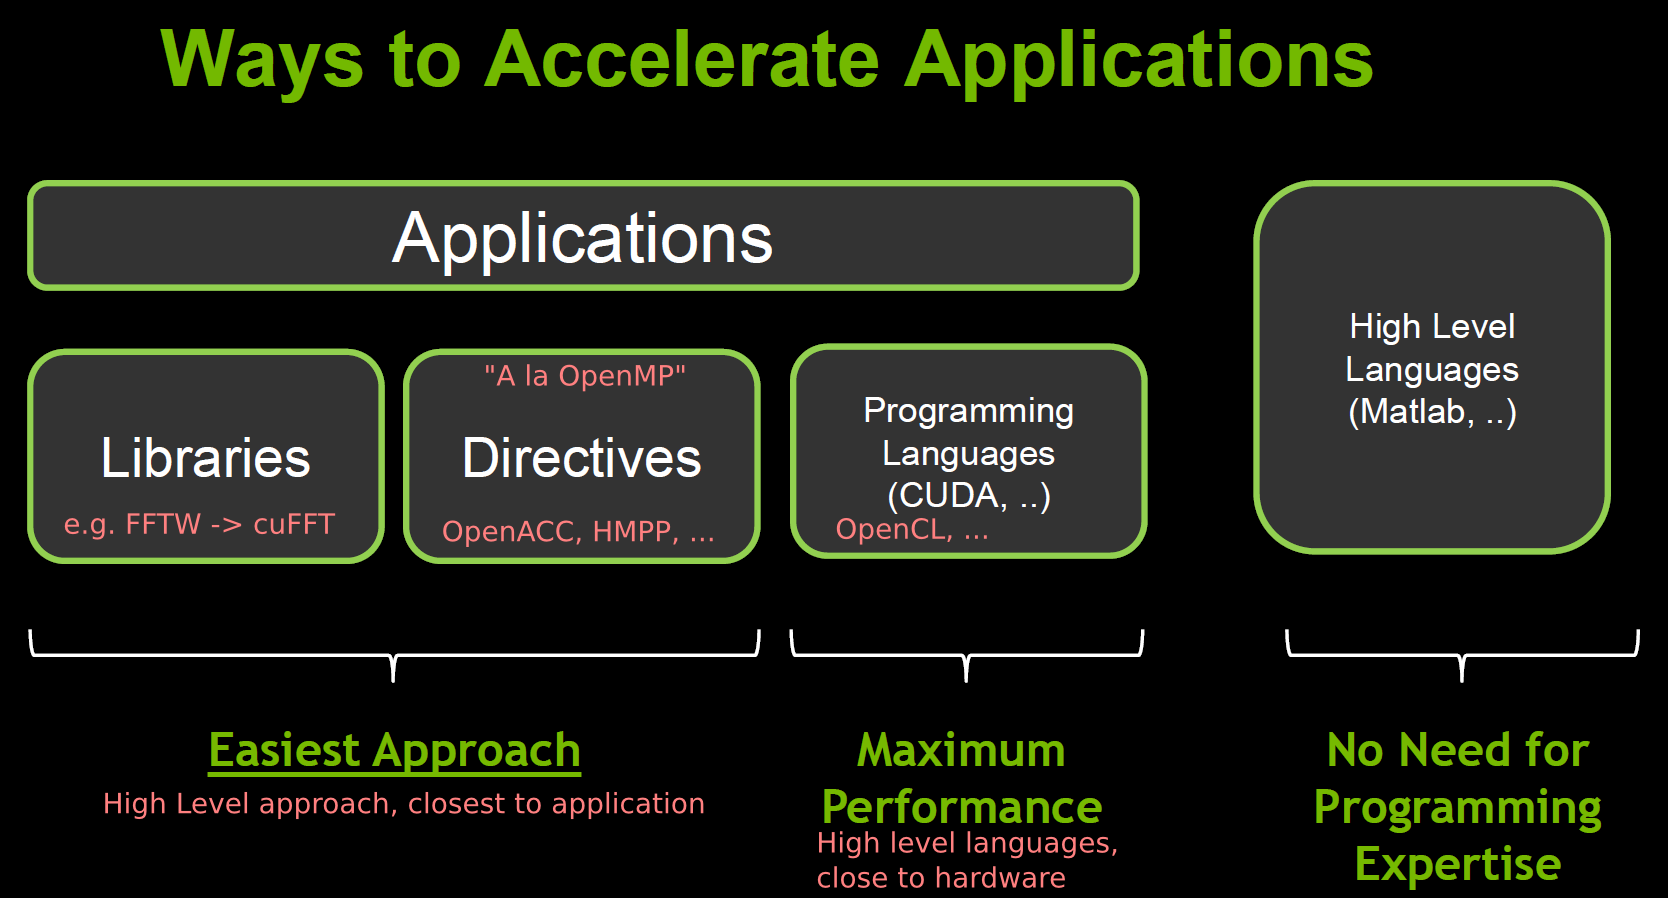
\includegraphics[height=5.0cm]{images/ways_to_accelerate_app2}
  \end{center}
  
  {\scriptsize reference: Axel Koehler, \myhref{http://www.hpcadvisorycouncil.com/events/2012/Switzerland-Workshop/Presentations/Day_2/6_NVIDIA.pdf}{NVIDIA, 2012}}

  Find a good trade-off between \textcolor{blue}{\textit{ease of approach}} and \textcolor{blue}{\textit{good performance}} on \textcolor{red}{\textbf{multiple architectures}}.
  
\end{frame}

%\input{hpc_software_engineer}

%\section{Historical perspective}
%\input{./historique_gpu_mini}
%%%%%%%%%%%%%%%%%%%%%%%%%%%%%%%%%%%%%%%%%%%%%%%%%%%%%%%%%%%%%%%%%%%%%%%% 
%%%%%%%%%%%%%%%%%%%%%%%%%%%%%%%%%%%%%%%%%%%%%%%%%%%%%%%%%%%%%%%%%%%%%%%% 
\begin{frame}
  \frametitle{Supercomputers architectures - TOP500}

  A Supercomputer is designed to be at bleeding edge of current technology.

  { Leading technology paths (to exascale) using \myhref{http://top500.org/lists/2013/11/}{TOP500} ranks (Nov. 2016)}
  \begin{itemize}
  \item \textcolor{blue}{\textbf{Multicore:}} Maintain complex cores, and replicate (x86, SPARC) (\#7, 10)
  \item \textcolor{blue}{\textbf{Manycore/Embedded:}} Use many simpler, low power cores from embedded (IBM BlueGene) (\#4, 9)
  \item \textcolor{darkgreen}{\textbf{Manycore/Sunway}} (\# 1)
  \item \textcolor{darkgreen}{\textbf{Manycore/Intel XeonPhi (1st and 2nd gen):}} Use many simpler cores with wide SIMD instructions, (\# 2, 5, 6)
  \item \textcolor{darkgreen}{\textbf{Massively Multithread/ GPU:}}  (\# 3, 8)
  \end{itemize}

  \textcolor{orange}{\textbf{Sunway Taihulight}} : programmed with \myhref{http://www.netlib.org/utk/people/JackDongarra/PAPERS/sunway-report-2016.pdf}{MPI+OpenACC}

  Next year, we might have supercomputers build with \textcolor{red}{\textbf{ARMv8}} CPU (From China, Japan, US,...), \textcolor{orange}{\textbf{DOE Coral machines}} (\textbf{NVidia GPU+IBM Power9, Intel KNL}), ...

\end{frame}

%%%%%%%%%%%%%%%%%%%%%%%%%%%%%%%%%%%%%%%%%%%%%%%%%%%%%%%%%%%%%%%%%%%%%%%% 
%%%%%%%%%%%%%%%%%%%%%%%%%%%%%%%%%%%%%%%%%%%%%%%%%%%%%%%%%%%%%%%%%%%%%%%% 
\begin{frame}
  \frametitle{About DOE Coral next generation computing facility}

  \begin{itemize}
  \item As part of \textcolor{orange}{\textbf{CORAL}} (Next gen supercomputers): \textbf{Center for Accelerated Application Readiness}
  \item Provide \textcolor{red}{\textbf{programming environments and tools}} that enable \textcolor{blue}{\textbf{portability}}
  \end{itemize}
  
  \begin{center}
    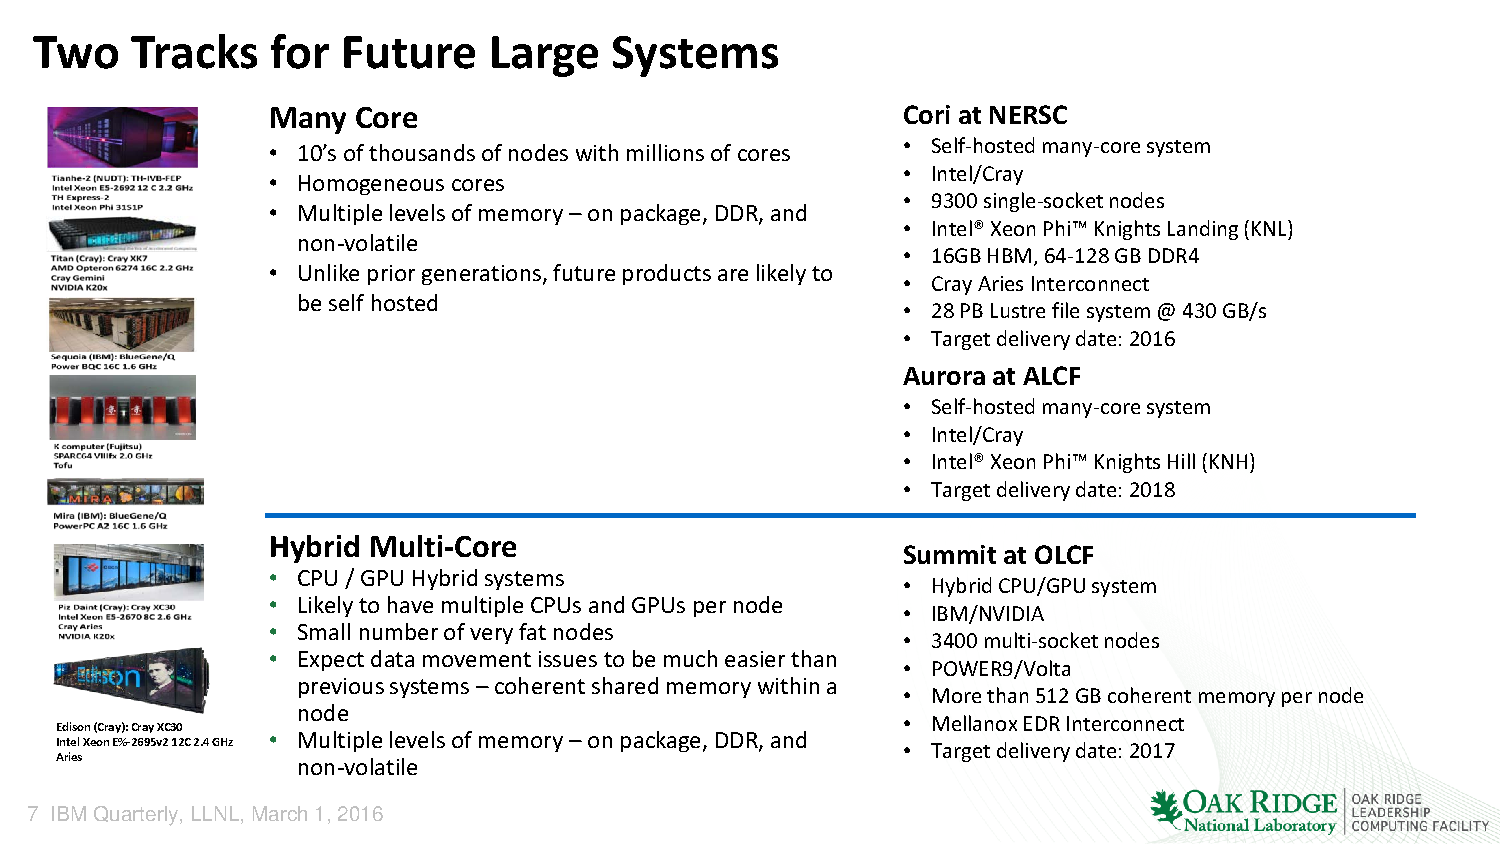
\includegraphics[height=5.5cm]{doc/perf_portability/1-02_Straatsma_7}
  \end{center}
  
\end{frame}

%%%%%%%%%%%%%%%%%%%%%%%%%%%%%%%%%%%%%%%%%%%%%%%%%%%%%%%%%%%%%%%%%%%%%%%% 
%%%%%%%%%%%%%%%%%%%%%%%%%%%%%%%%%%%%%%%%%%%%%%%%%%%%%%%%%%%%%%%%%%%%%%%% 
\begin{frame}
  \frametitle{HPC architectures - Trends - Who's driving ?}

  \begin{minipage}{0.55\linewidth}
    \begin{itemize}
    \item \textcolor{darkblue}{\textbf{Artificial Intelligence}} applications : e.g. \textbf{Japan} (ABCI: a 130 single precision PetaFlops system in late 2017) for Companies (book time for a fee)\\
      \textbf{AI Bridging Cloud Infrastructure}: goal is 43 (FP32) GigaFlops/Watt\\
    \item \textcolor{darkgreen}{\textbf{Energy efficiency}}, e.g. \myhref{https://www.nextplatform.com/2016/11/14/nvidias-saturn-v-dgx-1-cluster-stacks/}{Nvidia's DGX-1 node} server (1 Dual Xeon + 8 GPU P100) aimed at deep learning ($\sim 18$ (FP64) GigaFlops/Watt).
    \item \textbf{Several new hardware solutions} to come next year and after: Intel Knights Mill (XeonPhi, 3rd gen), FPGA (?) for dedicated specific applications, ... \textcolor{red}{$\Rightarrow$ \textbf{a good programing model !}}
    \end{itemize}    
  \end{minipage}
  %
  \begin{minipage}{0.4\linewidth}
    \begin{center}
      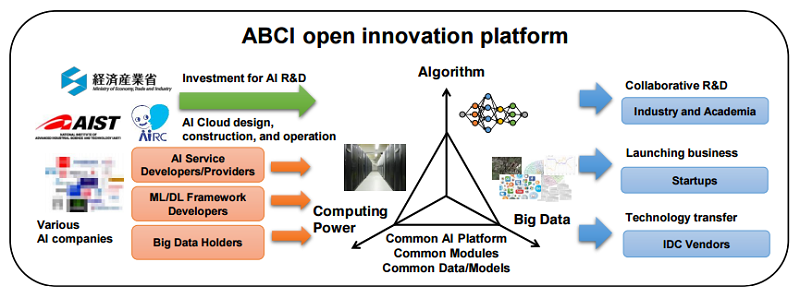
\includegraphics[width=5cm]{images/abci-innovation-800x298}
    \end{center}

    \begin{center}
      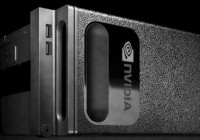
\includegraphics[width=3.5cm]{images/nvidia-dgx-1-bw-200x140}
    \end{center}
  \end{minipage}

  % \begin{itemize}
  % \item \textcolor{darkblue}{\textbf{Artificial Intelligence}} applications : e.g. \textbf{Japan} (ABCI: a 130 single precision PetaFlops system in late 2017) for Companies (book time for a fee)\\
  %   \textbf{AI Bridging Cloud Infrastructure}: goal is 43 (FP32) GigaFlops/Watt\\
  % \item \textcolor{darkgreen}{\textbf{Energy efficiency}}, e.g. \myhref{https://www.nextplatform.com/2016/11/14/nvidias-saturn-v-dgx-1-cluster-stacks/}{Nvidia's DGX-1 node} server (1 Dual Xeon + 8 GPU P100) aimed at deep learning ($\sim 18$ (FP64) GigaFlops/Watt).
  % \item Many new hardware solutions to come next year and after: Intel Knights Mill (XeonPhi, 3rd gen)
  % \end{itemize}

\end{frame}

%%%%%%%%%%%%%%%%%%%%%%%%%%%%%%%%%%%%%%%%%%%%%%%%%%%%%%%%%%%%%%%%%%%%%%%% 
%%%%%%%%%%%%%%%%%%%%%%%%%%%%%%%%%%%%%%%%%%%%%%%%%%%%%%%%%%%%%%%%%%%%%%%% 
\begin{frame}
  \frametitle{Supercomputer node architecture}

  \begin{center}
    \textbf{Multiples levels of hierarchy:}
    \begin{itemize}
    \item Need to aggregate the computing power of several 10 000 nodes !
    \item network efficiency: latency, bandwidth, topology
    \item memory: on-chip (cache), out-of-chip (DRAM), IO (disk)
    \item emmerging \textbf{hybrid programming model: MPI + X}
    \item \textcolor{red}{What is \textbf{X} ? OpenMP, OpenAcc, ..., \myhref{https://github.com/kokkos/kokkos}{Kokkos}, \myhref{https://github.com/llnl/raja}{RAJA}, ...}
    \item \textcolor{blue}{Even at node level MPI+X is required:} e.g. KNL
    \end{itemize}
  \end{center}

  \begin{figure}
    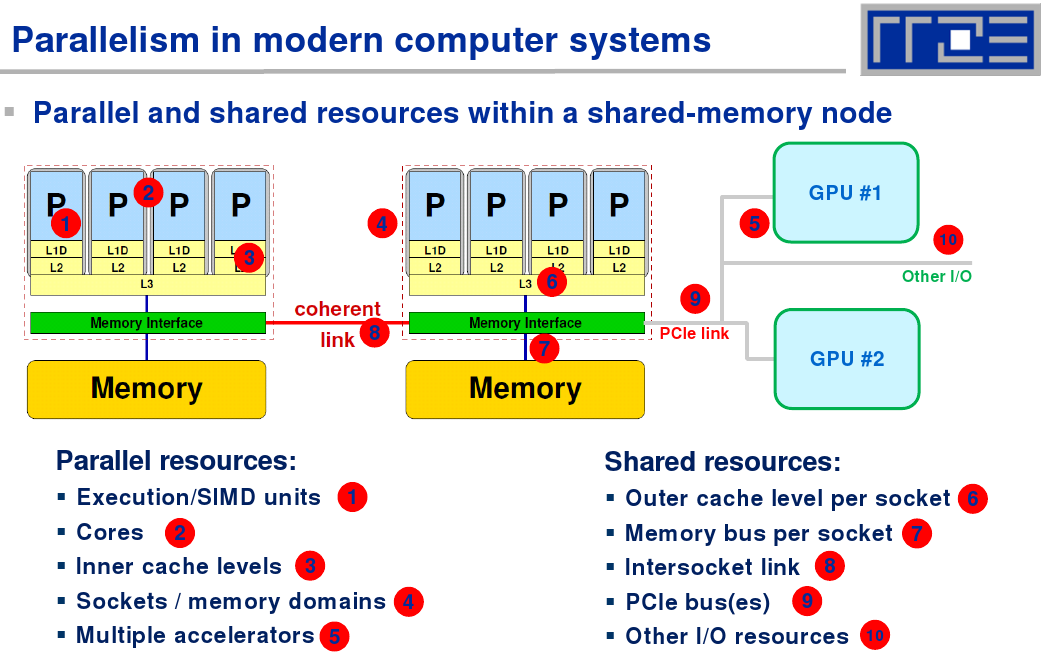
\includegraphics[width=5cm]{images/multicore_hardware}
    \caption{\scriptsize{Multi-core node summary,
        source: multicore tutorial (SC12) by G. Hager and G. Wellein}}
  \end{figure}
  
\end{frame}

%%%%%%%%%%%%%%%%%%%%%%%%%%%%%%%%%%%%%%%%%%%%%%%%%%%%%%%%%%%%%%%%%%%%%%%% 
%%%%%%%%%%%%%%%%%%%%%%%%%%%%%%%%%%%%%%%%%%%%%%%%%%%%%%%%%%%%%%%%%%%%%%%% 
% \begin{frame}
%   \frametitle{More heterogeneous  future...}

%   \begin{figure}
%     \includegraphics[height=6.5cm]{images/kokkos_heterogeneous}
%     \caption{
%       source: kokkos tutorial (GTC2014) by Carter Edwards}
%   \end{figure}
  
% \end{frame}


%%%%%%%%%%%%%%%%%%%%%%%%%%%%%%%%%%%%%%%%%%%%%%%%%%%%%%%%%%%%%%%%%%%%%%%% 
%%%%%%%%%%%%%%%%%%%%%%%%%%%%%%%%%%%%%%%%%%%%%%%%%%%%%%%%%%%%%%%%%%%%%%%% 
% \begin{frame}
%   \frametitle{What is a supercomputer ?}
  
%   % Power Efficiency over time
%   \begin{figure}
%     \includegraphics[height=6cm]{images/power_efficiency_horst_simon}
%     \caption{\myhref{http://www.extremetech.com/computing/155941-supercomputing-director-bets-2000-that-we-wont-have-exascale-computing-by-2020}{Horst Simon, LBNL}}
%   \end{figure}
  
% \end{frame}


%\section{CUDA Hardware / Software}
%\input{./cuda_hardware_mini}
%\input{../cuda_example}

\section{Performance Portability}

%%%%%%%%%%%%%%%%%%%%%%%%%%%%%%%%%%%%%%%%%%%%%%%%%%%%%%%%%%%%%%%%%%%%%%%% 
%%%%%%%%%%%%%%%%%%%%%%%%%%%%%%%%%%%%%%%%%%%%%%%%%%%%%%%%%%%%%%%%%%%%%%%% 
\begin{frame}
  \frametitle{Performance portability}

  \begin{itemize}
  \item \textbf{Developing / maintaining} a \textcolor{red}{\textbf{separate}} implementation of an application for each \textbf{new hardware platform} (Intel KNL, Nvidia GPU, ARMv8, ...) is \textcolor{red}{\textbf{less and less realistic}}
  \item \textbf{Identical code} will never perform \textbf{optimally} on all platforms~\footnote{source: Matt Norman, \myhref{http://waccpd.org/wp-content/uploads/2016/04/WACCPD_2016_Norman.pdf}{WACCPD 2016}}
  \item Is it possible to have a \textcolor{blue}{\textbf{single set of source codes}} that can be compiled for different hardware targets ?
\only<1>{
  \item Performance portability should be understood as a single source code base with
    \begin{itemize}
    \item \textcolor{darkgreen}{\textbf{good}} performance on different architectures
    \item a relatively \textcolor{darkgreen}{\textbf{small amount of effort}} required to tune app performance from one architecture to another.\\
      {\tiny source \myurl{http://www.nersc.gov/research-and-development/application-readiness-across-doe-labs}}
    \end{itemize}
  }
  \only<2>{
  \item \textcolor{darkgreen}{\bf performance portability} is achieved when software implementation
    \begin{itemize}
    \item compiles and runs on {\bf multiple architectures},
    \item obtains performant {\bf memory access patterns} across architectures,
    \item can {\bf leverage architecture-specific features} where possible.
    \end{itemize}
  }
  \end{itemize}
  \vfill
\end{frame}

%%%%%%%%%%%%%%%%%%%%%%%%%%%%%%%%%%%%%%%%%%%%%%%%%%%%%%%%%%%%%%%%%%%%%%%% 
%%%%%%%%%%%%%%%%%%%%%%%%%%%%%%%%%%%%%%%%%%%%%%%%%%%%%%%%%%%%%%%%%%%%%%%% 
\begin{frame}
  \frametitle{Performance portability issue}
  \textcolor{orange}{\large \textbf{Developper productivity versus optimization}}

  \begin{itemize}
  \item \textcolor{red}{\bf Taking into account hardware details is a hard job}
    \begin{itemize}
    \item CPU vector length: 256 bits (8 \textit{vector threads})\\
      \textcolor{violet}{Heavily cache-based}
    \item KNL vector length: 512 bits  x  2 (16-32 \textit{vector threads})\\
      \textcolor{violet}{Moderately cache-based, some latency/bandwidth hiding}
    \item GPU vector length: 65 536 bit (2048 \textit{GPU vector threads})\\
      \textcolor{violet}{Less cache-based, heavy on latency/bandwidth hiding}
    \end{itemize}
  \item \textcolor{darkgreen}{\bf Find ways of writing codes that avoid optimization blockers}\\
    $\Rightarrow$ Constructs that can be used to express operations without going into details
  \end{itemize}
\end{frame}

%%%%%%%%%%%%%%%%%%%%%%%%%%%%%%%%%%%%%%%%%%%%%%%%%%%%%%%%%%%%%%%%%%%%%%%% 
%%%%%%%%%%%%%%%%%%%%%%%%%%%%%%%%%%%%%%%%%%%%%%%%%%%%%%%%%%%%%%%%%%%%%%%% 
\begin{frame}
  \frametitle{Performance portability issue : algorithmic patterns}

  \begin{itemize}
  \item Is it possible to have a single set of source codes that can be compiled for different hardware targets ?
  \item \textcolor{red}{\textbf{Low-level native language:}} OpenCL, CUDA, ...
  \item \textcolor{orange}{\textbf{Directive approach (code annotations)}} for multicore/GPU, ...: 
    \begin{itemize}
    \item \myhref{http://www.openmp.org/}{OpenMP} 4.5 (Clang, GNU, PGI, ...)
    \item \myhref{http://www.openacc.org/}{OpenACC} 2.5 (PGI, GNU, ...)
    \end{itemize}
  \item \textcolor{darkgreen}{\textbf{Other high-level library-based approaches}} (mostly c++-based, à la TBB):
    \begin{itemize}
    \item Some provide STL-like algorithmics patterns (e.g. \myhref{https://github.com/thrust/thrust}{Thrust} is CUDA-based with backends for other archs, \myhref{https://github.com/nsubtil/lift.git}{lift}, \myhref{https://github.com/arrayfire/arrayfire}{arrayFire} (numerical libraries, language wrappers, ...))
    \item \myhref{https://github.com/kokkos/kokkos}{Kokkos}, \myhref{https://github.com/LLNL/RAJA}{RAJA}, \myhref{https://github.com/ComputationalRadiationPhysics/alpaka}{Alpaka}, \myhref{https://github.com/dash-project/dash}{Dash-project}, \myhref{https://github.com/agency-library/agency}{agency}, ...
    \item Cross-platform frameworks
      \begin{itemize}
      \item \myhref{http://charmplusplus.org/}{Chamm++}: message-driven execution, task and data migration, distributed load-balancing, ...
      \item \myhref{https://github.com/STEllAR-GROUP/hpx}{hpx} (heavy use of new c++ standards (11,14,17): \texttt{std::future, std::launch::async}, distributed parallelism, ...)
      \item \myhref{https://www.khronos.org/sycl}{SYCL} (Khronos Group \textit{standard}), one implementation by \myhref{https://www.codeplay.com/products/computesuite/computecpp}{CodePlay}, by \myhref{https://github.com/keryell/triSYCL}{Keryell/Xilinx}, ..., \myhref{https://github.com/KhronosGroup/SyclParallelSTL}{parallel STL}, wide hardware targets (CPU, GPU, FPGA, ...)
      \end{itemize}
    \end{itemize}
  {\small \item \textcolor{darkblue}{\textbf{Use an embedded Domain Specific Language (DSL)}}
    \begin{itemize}
    \item \myhref{http://halide-lang.org/}{Halide} (for image processing),
    \item \myhref{http://www.nabla-lang.org/}{NABLA} (for HPC, developped at CEA, PDE mesh+particules apps)
    \end{itemize}}
  \end{itemize}

  {\small \myhref{https://www.khronos.org/assets/uploads/developers/library/2016-supercomputing/SC16-compareSYCL-Michael-Wong_Nov16.pdf}{SC16-compareSYCL-Michael-Wong\_Nov16.pdf}}
  
\end{frame}


%%%%%%%%%%%%%%%%%%%%%%%%%%%%%%%%%%%%%%%%%%%%%%%%%%%%%%%%%%%%%%%%%%%%%%%% 
%%%%%%%%%%%%%%%%%%%%%%%%%%%%%%%%%%%%%%%%%%%%%%%%%%%%%%%%%%%%%%%%%%%%%%%% 
\begin{frame}
  \frametitle{Performance portability issue : memory management}

  \begin{itemize}
  \item Right now \textbf{directives-based approaches} focus on algorithmic pattern, and less on memory layout (might change in the near future, at least in OpenMP).
  \item CPU and GPU for example require \textcolor{blue}{\textbf{different memory layout}} for \textcolor{darkgreen}{\textbf{maximun performance:}}
    \begin{itemize}
    \item vectorization on CPU
    \item memory coalescence on GPU
    \end{itemize}
  \item Some libraries like \myhref{https://github.com/kokkos/kokkos}{Kokkos} promote \textcolor{blue}{\textbf{memory layout}} as a \textcolor{darkgreen}{\textbf{major concern}}
  \end{itemize}

  \begin{center}
    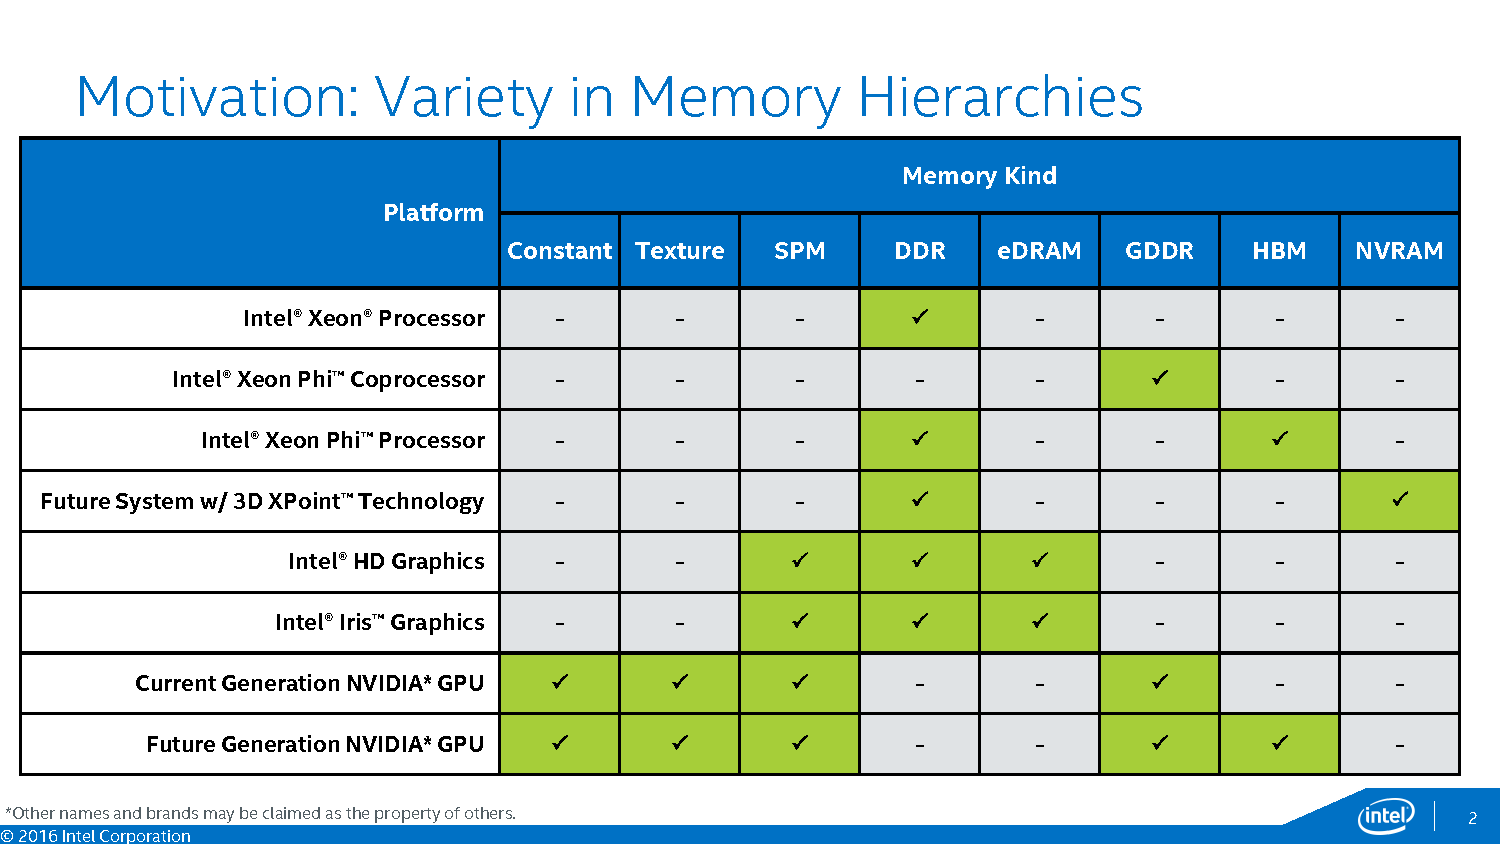
\includegraphics[width=6cm]{doc/openmp/omp_memory}
  \end{center}


\end{frame}



\subsection{Directives: OpenACC / OpenMP}

%%%%%%%%%%%%%%%%%%%%%%%%%%%%%%%%%%%
%%%%%%%%%%%%%%%%%%%%%%%%%%%%%%%%%%%
\begin{frame}
  \frametitle{Programming with structured parallel patterns}

  \begin{minipage}{0.7\linewidth}
    \begin{itemize}
    \item \textcolor{red}{\textbf{pattern}} : \textbf{a basic structural entity of an algorithm}
      % http://parallelbook.com/sites/parallelbook.com/files/SC13_20131117_Intel_McCool_Robison_Reinders_Hebenstreit.pdf
    \item book \myhref{http://parallelbook.com/}{Structured Parallel Programming:} \myhref{http://parallelbook.com/}{Patterns for Efficient Computation}
    \end{itemize}
  \end{minipage}
  \hfill{}
  \begin{minipage}{0.25\linewidth}
    \vfill{}
    %\begin{center}
    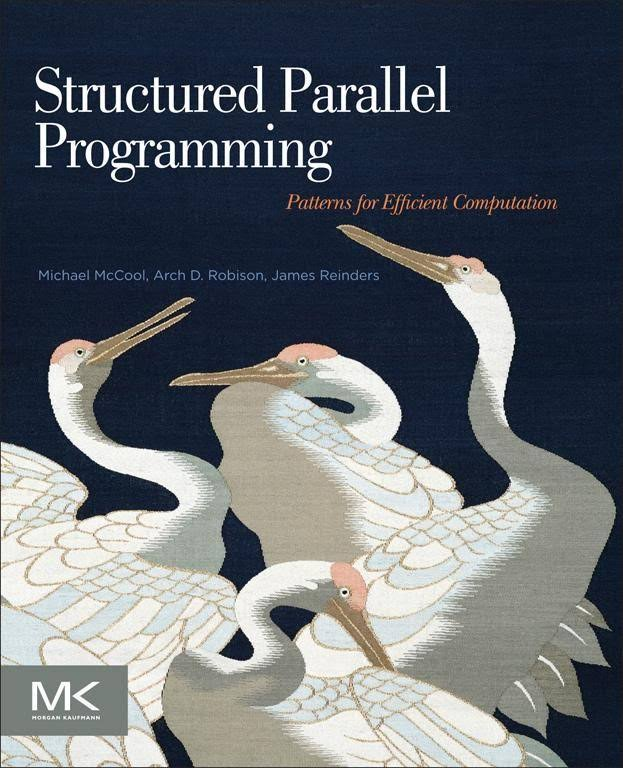
\includegraphics[width=2.5cm]{images/structured_parallel_programming}
    %\end{center}
  \end{minipage}

  \begin{itemize}
    \item implementation: Intel TBB, OpenMP, OpenACC and many others
    \item  {\small \myhref{https://sharepoint.campus.rwth-aachen.de/units/rz/HPC/public/Shared\%20Documents/WienkeEtAl_OpenACC-OpenMP-PatternComparison.pdf}{OpenMP/OpenAcc for GPU/XeonPhi: pattern-based comparison}: map, stencil, reduce, scan, fork-join, superscalar sequence, parallel update}
      % map -> SAXPY
  \end{itemize}

  {\scriptsize
  reference:\\
  \myhref{http://link.springer.com/chapter/10.1007/978-3-319-09873-9_68}{A Pattern-Based Comparison of OpenACC and OpenMP for Accelerator Computing}}

\end{frame}

%%%%%%%%%%%%%%%%%%%%%%%%%%%%%%%%%%%
%%%%%%%%%%%%%%%%%%%%%%%%%%%%%%%%%%%
\begin{frame}
  \frametitle{Programming with structured parallel patterns}

  \begin{center}
  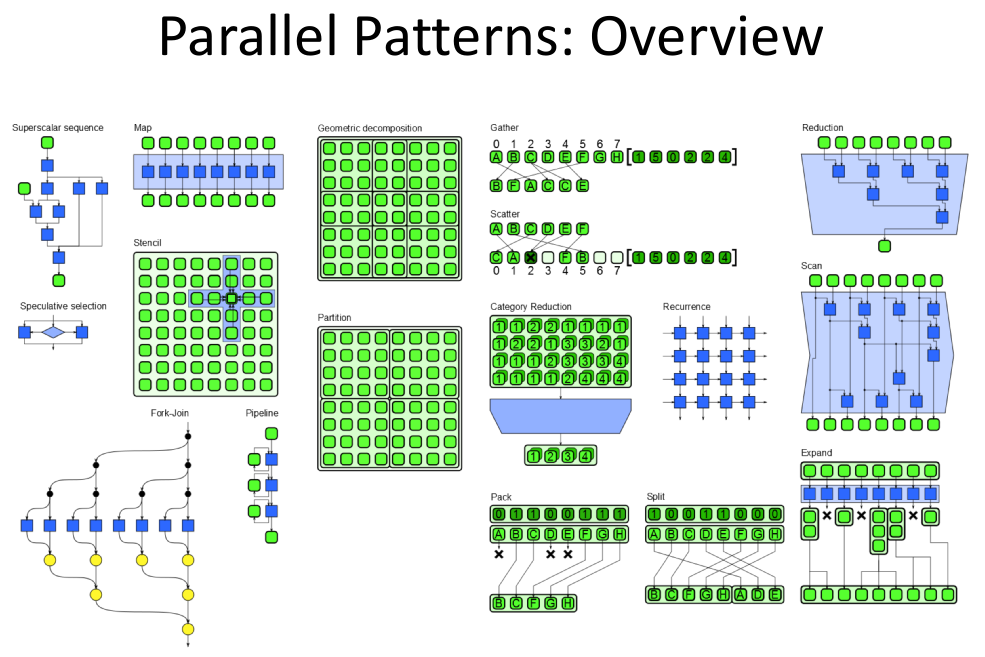
\includegraphics[width=9cm]{images/parallel_patterns2}
  \end{center}

  {\scriptsize
  reference: Structured Parallel Programming with Patterns, SC13 tutorial, by M. Hebenstreilt, J. Reinders, A. Robison, M. McCool}

\end{frame}


\subsection{(Active) libraries}

%%%%%%%%%%%%%%%%%%%%%%%%%%%%%%%%%%%%%%%%%%%%%%%%%%%%%%%%%%%%%%%%%%% 
%%%%%%%%%%%%%%%%%%%%%%%%%%%%%%%%%%%%%%%%%%%%%%%%%%%%%%%%%%%%%%%%%%% 
%%%%%%%%%%%%%%%%%%%%%%%%%%%%%%%%%%%%%%%%%%%%%%%%%%%%%%%%%%%%%%%%%%% 
\begin{frame}
  \frametitle{Future of accelerator programming}

  \begin{itemize}
  \item \textcolor{red}{\textbf{passive libraries:}} a collection of subroutines
  \item \textcolor{blue}{\textbf{active libraires:}} take an active role in compilation (specialize algorithms, tune themselves for target architecture).
  \end{itemize}

  \begin{center}
    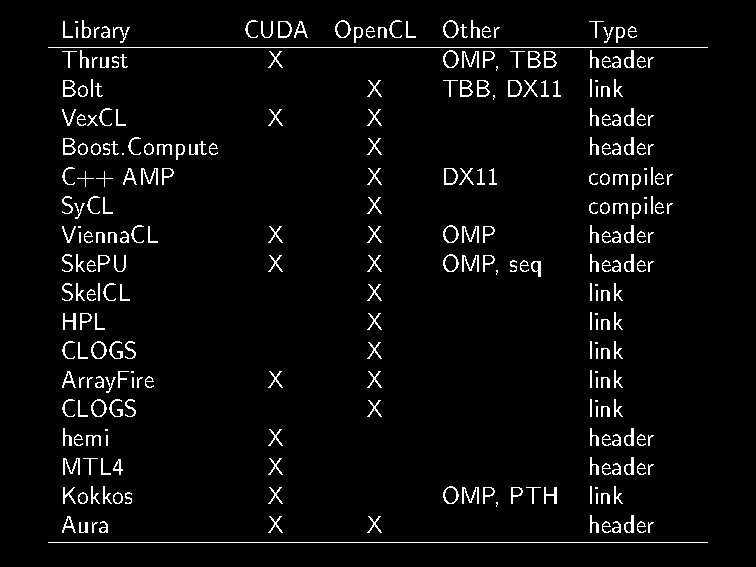
\includegraphics[width=6cm]{images/acc_prog_cpp.pdf}
  \end{center}
  
  reference: \myhref{http://www.soa-world.de/echelon/wp-content/uploads/2014/05/CppNow2014_Future_of_Accelerator_Programming.pdf}{The Future of
    Accelerator Programming in C++, S. Schaetz, May 2014}
  
\end{frame}

%%%%%%%%%%%%%%%%%%%%%%%%%%%%%%%%%%%%%%%%%%%%%%%%%%%%%%%%%%%%%%%%%%% 
%%%%%%%%%%%%%%%%%%%%%%%%%%%%%%%%%%%%%%%%%%%%%%%%%%%%%%%%%%%%%%%%%%% 
%%%%%%%%%%%%%%%%%%%%%%%%%%%%%%%%%%%%%%%%%%%%%%%%%%%%%%%%%%%%%%%%%%% 
% \begin{frame}
%   \frametitle{Future of accelerator programming}

%   \begin{itemize}
%   \item \textbf{Coordination:}
%     \begin{itemize}
%     \item concurrency: asynchronicity, data dependency graph
%     \item memory management (explicit ? implicit ?) / memory layout (SoA, AoS, unordered map, Morton-index, ...)
%     \end{itemize}
    
%   \item \textbf{Computation:}
%     \begin{itemize}
%     \item parallel primitives
%     \item custom accelerator functions
%     \item numerical analysis
%     \item performance portability
%     \item kernel-space exploration / tuning
%     \end{itemize}
%   \end{itemize}

%   reference: \myhref{http://www.soa-world.de/echelon/wp-content/uploads/2014/05/CppNow2014_Future_of_Accelerator_Programming.pdf}{The Future of
%     Accelerator Programming in C++, S. Schaetz, May 2014}
  
% \end{frame}

%%%%%%%%%%%%%%%%%%%%%%%%%%%%%%%%%%%%%%%%%%%%%%%%%%%%%%%%%%%%%%%%%%% 
%%%%%%%%%%%%%%%%%%%%%%%%%%%%%%%%%%%%%%%%%%%%%%%%%%%%%%%%%%%%%%%%%%% 
%%%%%%%%%%%%%%%%%%%%%%%%%%%%%%%%%%%%%%%%%%%%%%%%%%%%%%%%%%%%%%%%%%% 
\begin{frame}
  \frametitle{Complex memory layout for performance}

  \begin{itemize}
  \item How to improve \textcolor{red}{\textbf{space (memory) locality}} in algorithm implementations ?
  \item \textbf{\textit{High Performance Parallelism Pearls}}, \textcolor{darkgreen}{\textbf{Morton order to improve memory locality}}, by Kerry Evans (INTEL), chap. 28
  \item \textbf{matrix transpose}, \textbf{dense matrix multiplication} on Xeon, KNC
  \item Same feature used in some Adaptive Mesh Refinement PDE solver.
  \end{itemize}

  
  \begin{center}
    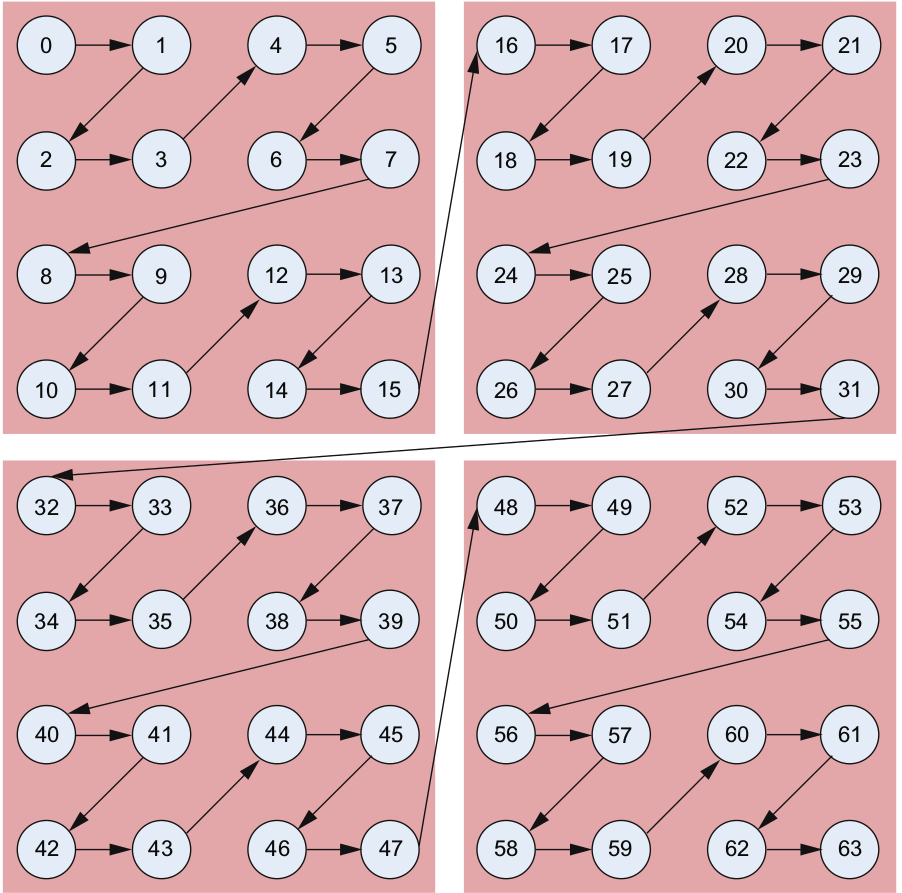
\includegraphics[width=3.5cm]{images/c28_morton_order}
    \hfill
    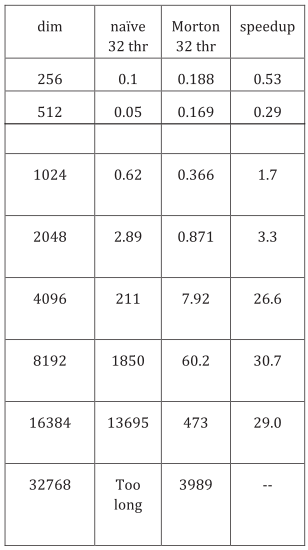
\includegraphics[height=3.5cm]{images/c28_MatrixMult_xeon1}
    \hfill
    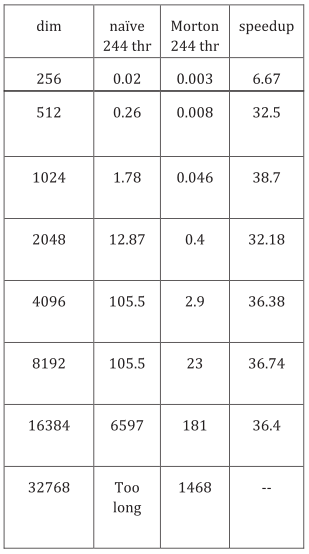
\includegraphics[height=3.5cm]{images/c28_MatrixMult_MIC}
  \end{center}

\end{frame}


\subsection{Asynchronous tasking}

%%%%%%%%%%%%%%%%%%%%%%%%%%%%%%%%%%%%%%%%%%%%%%%%%%%%%%%%%%%%%%%%%%%%%%%% 
%%%%%%%%%%%%%%%%%%%%%%%%%%%%%%%%%%%%%%%%%%%%%%%%%%%%%%%%%%%%%%%%%%%%%%%% 
\begin{frame}
  \frametitle{The future of portable asynchonous tasking}

  {\large \textcolor{darkgreen}{{\bf HiHAT initiative:} Hierarchical Heterogenous Asynchronous Tasking}}

  \begin{itemize}
  \item for Runtime frameworks developpers + HW vendors
  \item<1> Tasking frameworks
  \item<2> Fonctionalities
  \end{itemize}
  
  \only<1>{
    \begin{center}
      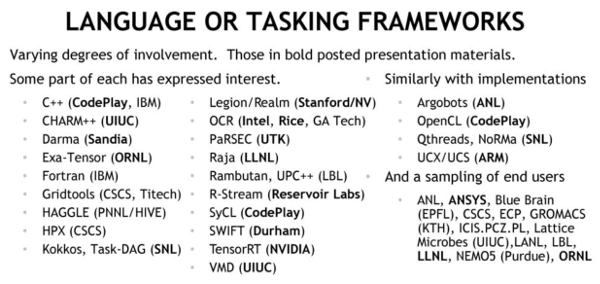
\includegraphics[height=5.0cm]{doc/perf_portability/hihat/hihat_1b}
    \end{center}
  }
  \only<2>{
    \begin{center}
      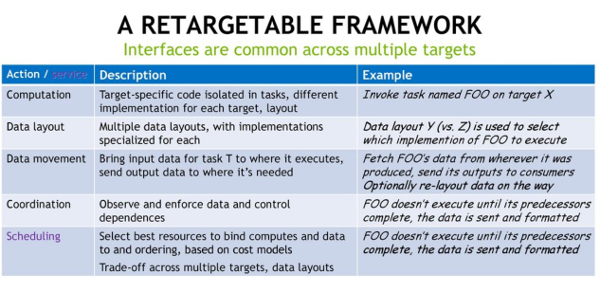
\includegraphics[height=5.0cm]{doc/perf_portability/hihat/hihat_2b}
    \end{center}
  }

  {\small
    reference \myhref{https://wiki.modelado.org/images/5/54/HiHAT_Mini-Summit_17_Overview.pdf}{HiHAT\_Mini-Summit\_17\_Overview.pdf}\\
    reference \myurl{http://slideplayer.com/slide/12990108/}
  }

\end{frame}

%%%%%%%%%%%%%%%%%%%%%%%%%%%%%%%%%%%%%%%%%%%%%%%%%%%%%%%%%%%%%%%%%%%%%%%% 
%%%%%%%%%%%%%%%%%%%%%%%%%%%%%%%%%%%%%%%%%%%%%%%%%%%%%%%%%%%%%%%%%%%%%%%% 
\begin{frame}
  \frametitle{AMT : Asynchonous Many Task frameworks}
  
  \begin{itemize}
  \item \myhref{https://github.com/StanfordLegion/legion}{Legion} (Stanford)
  \item \myhref{http://starpu.gforge.inria.fr/}{StarPU} (Inria Bordeaux)
  \item \myhref{https://share-ng.sandia.gov/darma/}{DARMA} (Sandia NL)
    %\myurl{http://theory.stanford.edu/~aiken/WEST/Talks/Darma.pdf}\\
    %\myurl{https://indico.sissa.it/event/8/contribution/64/material/slides/0.pdf}
    %\myurl{https://share-ng.sandia.gov/darma/_assets/documents/ECP-Review-2016-DARMA.pdf}
  \item \myhref{http://charmplusplus.org/}{Charm++} (Univ. Illinois, Urban Champain)
  \item \myhref{http://uintah.sci.utah.edu/}{Uintah}
  \item \myhref{https://github.com/STEllAR-GROUP/hpx}{HPX}
  \end{itemize}

  \myhref{https://share-ng.sandia.gov/darma/_assets/documents/Sandia2015_AMT_RTS_L2.pdf}{Comparative analysis of Legion, Charm++, Uintah}

\end{frame}


\section{Kokkos introduction}

\subsection{Kokkos basics}

%%%%%%%%%%%%%%%%%%%%%%%%%%%%%%%%%%%%%%%%%%%%%%%%%%%%%%%%%%%%%%%%%%% 
%%%%%%%%%%%%%%%%%%%%%%%%%%%%%%%%%%%%%%%%%%%%%%%%%%%%%%%%%%%%%%%%%%% 
%%%%%%%%%%%%%%%%%%%%%%%%%%%%%%%%%%%%%%%%%%%%%%%%%%%%%%%%%%%%%%%%%%% 
\begin{frame}
  \frametitle{Kokkos: a programming model for performance portability}

  \only<1>{
    \begin{itemize}
    \item \textcolor{blue}{\textbf{Kokkos}} is a \textbf{C++ library} with \textcolor{red}{\textbf{parallel algorithmic patterns}} AND \textcolor{red}{\textbf{data containers}} for \textcolor{blue}{\textbf{node-level parallelism}}.
    \item Implementation relies heavily on \textbf{meta-programing} to derive native low-level code (OpenMP, Pthreads, CUDA, ...) and adapt data structure memory layout at compile-time
    \item Core developers at \textcolor{violet}{\textbf{SANDIA NL}} (\textbf{H.C. Edwards, C. Trott})
    \end{itemize}
  }
  \only<2>{
    \begin{itemize}
    \item \textcolor{darkgreen}{\textbf{Open source}}, \myurl{https://github.com/kokkos/kokkos}
    \item Primarily developped as a base building layer for \textbf{generic high-performance parallel linear algebra} in \myhref{https://github.com/trilinos/Trilinos}{Trilinos}
    \item Also used in molecular dynamics code, e.g. \myhref{http://lammps.sandia.gov/}{LAMMPS}
    \item Goal: \textcolor{orange}{\textbf{ISO/C++ 2020 Standard}} subsumes Kokkos abstractions~\footnote{see mdspan proposal \myurl{https://github.com/kokkos/array_ref}}
    \end{itemize}
  }
  \begin{center}
    \includegraphics<1-2>[width=6cm]{doc/perf_portability/kokkos_summary}
  \end{center}

\end{frame}

%%%%%%%%%%%%%%%%%%%%%%%%%%%%%%%%%%%%%%%%%%%%%%%%%%%%%%%%%%%%%%%%%%% 
%%%%%%%%%%%%%%%%%%%%%%%%%%%%%%%%%%%%%%%%%%%%%%%%%%%%%%%%%%%%%%%%%%% 
%%%%%%%%%%%%%%%%%%%%%%%%%%%%%%%%%%%%%%%%%%%%%%%%%%%%%%%%%%%%%%%%%%% 
\begin{frame}
  \frametitle{Kokkos: a programming model for performance portability}

  {\large \textcolor{blue}{\textbf{Kokkos abstract concepts}}}

  \begin{itemize}
  \item \textbf{Execution patterns (what):}\\
    \textcolor{darkgreen}{parallel\_for, parallel\_reduce, ...}
  \item \textbf{Execution policy (how):}\\
    \textcolor{darkgreen}{range iterations, teams of threads, ...}
  \item \textbf{Execution space (where):}\\
    \textcolor{darkgreen}{OpenMP, PThreads, CUDA, numa, ...}
  \item \textbf{Memory space: data containers} with architecture adapted memory layout\\
    {\small \textcolor{darkgreen}{\texttt{Kokkos::View, Kokkos::DualView, Kokkos::UnorderedMap,...}}}
  \item \textbf{Memory layout:} (important for vectorization, memory coalescence, ...)\\
    \textcolor{darkgreen}{row-major, column-major, AoS, SoA, ...}\\
    $data(i,j,k)$ \textcolor{red}{architecture aware}.
  \end{itemize}
  
  {\scriptsize reference: \myhref{https://cfwebprod.sandia.gov/cfdocs/CompResearch/docs/2016-04-Kokkos-SIAM-PP.pdf}{Kokkos: Manycore programmability and performance portability, SIAM conference, Paris, 2016}}

\end{frame}

%%%%%%%%%%%%%%%%%%%%%%%%%%%%%%%%%%%%%%%%%%%%%%%%%%%%%%%%%%%%%%%%%%% 
%%%%%%%%%%%%%%%%%%%%%%%%%%%%%%%%%%%%%%%%%%%%%%%%%%%%%%%%%%%%%%%%%%% 
%%%%%%%%%%%%%%%%%%%%%%%%%%%%%%%%%%%%%%%%%%%%%%%%%%%%%%%%%%%%%%%%%%% 
\begin{frame}
  \frametitle{Kokkos: a programming model for performance portability}

  \begin{center}
    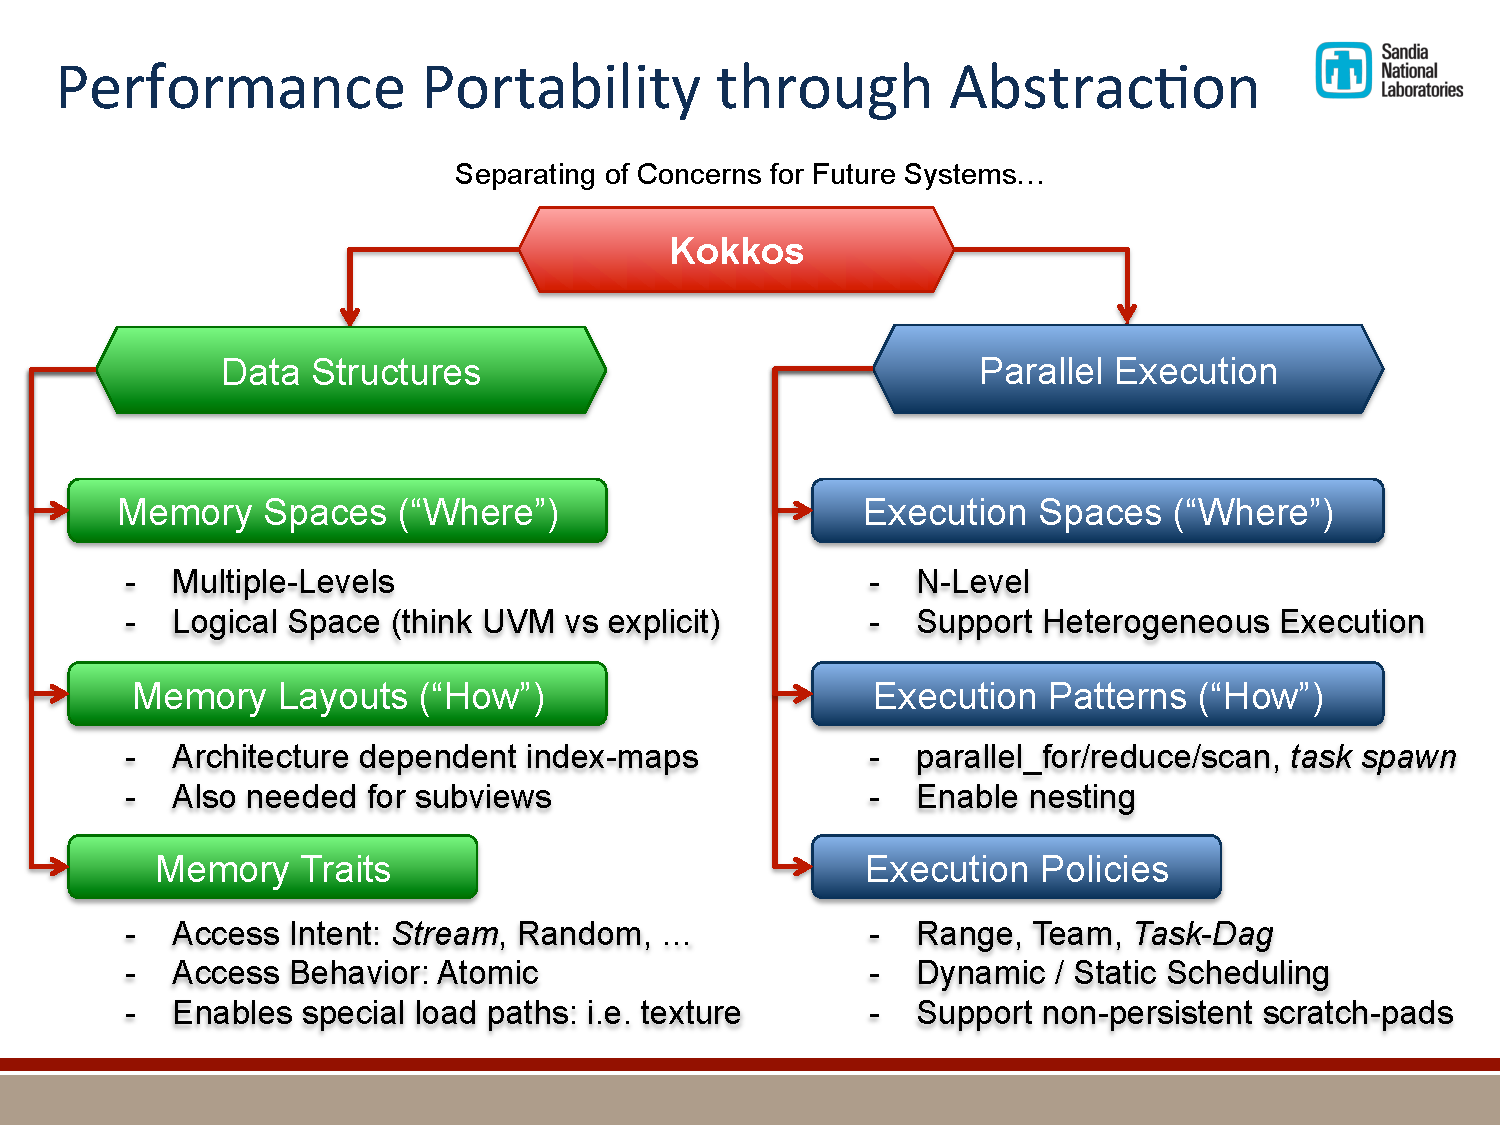
\includegraphics[width=8.5cm]{images/Kokkos-Multi-CoE_slide3}
  \end{center}

  {\small reference: \myurl{https://cfwebprod.sandia.gov/cfdocs/CompResearch/docs/Kokkos-Multi-CoE.pdf}}

\end{frame}

%%%%%%%%%%%%%%%%%%%%%%%%%%%%%%%%%%%%%%%%%%%%%%%%%%%%%%%%%%%%%%%%%%% 
%%%%%%%%%%%%%%%%%%%%%%%%%%%%%%%%%%%%%%%%%%%%%%%%%%%%%%%%%%%%%%%%%%% 
%%%%%%%%%%%%%%%%%%%%%%%%%%%%%%%%%%%%%%%%%%%%%%%%%%%%%%%%%%%%%%%%%%% 
\begin{frame}
  \frametitle{Kokkos: Sparse Matrix-Vector Multiply}

  \begin{center}
    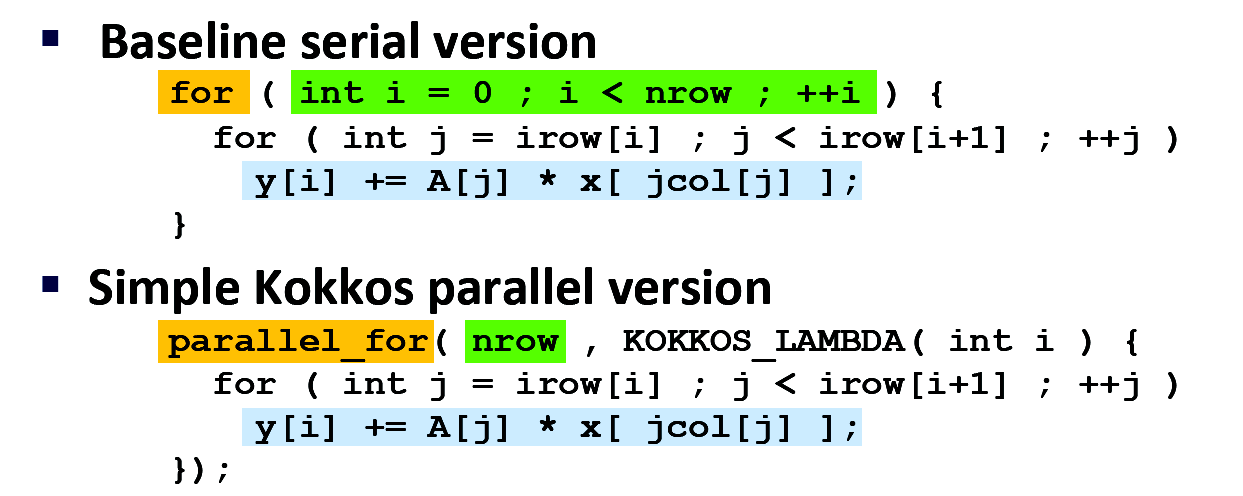
\includegraphics[width=8.5cm]{doc/perf_portability/kokkos_spmv}
  \end{center}

  \begin{itemize}
  \item Execution pattern: \textcolor{orange}{\textbf{parallel for}}
  \item Execution policy: \textcolor{darkgreen}{\textbf{range iteration}}
  \item Execution space: default (defined at compiled time)
  \item \textcolor{cyan}{\textbf{Work to do can be}}
    \begin{itemize}
    \item A \textbf{Lambda \textit{anonymous} function}, convenient for short loop bodies
    \item A \textbf{C++ class functor}, maximun flexibility
    \end{itemize}
  \end{itemize}
\end{frame}


%%%%%%%%%%%%%%%%%%%%%%%%%%%%%%%%%%%%%%%%%%%%%%%%%%%%%%%%%%%%%%%%%%% 
%%%%%%%%%%%%%%%%%%%%%%%%%%%%%%%%%%%%%%%%%%%%%%%%%%%%%%%%%%%%%%%%%%% 
%%%%%%%%%%%%%%%%%%%%%%%%%%%%%%%%%%%%%%%%%%%%%%%%%%%%%%%%%%%%%%%%%%% 
% \begin{frame}
%   \frametitle{Kokkos: a programming model for performance portability}
% \end{frame}

%%%%%%%%%%%%%%%%%%%%%%%%%%%%%%%%%%%%%%%%%%%%%%%%%%%%%%%%%%%%%%%%%%% 
%%%%%%%%%%%%%%%%%%%%%%%%%%%%%%%%%%%%%%%%%%%%%%%%%%%%%%%%%%%%%%%%%%% 
%%%%%%%%%%%%%%%%%%%%%%%%%%%%%%%%%%%%%%%%%%%%%%%%%%%%%%%%%%%%%%%%%%% 
% \begin{frame}
%   \frametitle{Future of accelerator programming: Kokkos among other}

%   \begin{center}
%     \includegraphics[width=8cm]{images/kokkos1}
%   \end{center}

%   {\scriptsize
%   reference: slides by Edwards, Trott, Sunderland (SANDIA) at GTC2014
%   \myhref{http://on-demand.gputechconf.com/gtc/2014/presentations/S4213-kokkos-manycore-device-perf-portability-library-hpc-apps.pdf}{Kokkos, a Manycore Device Performance Portability Library for C++ HPC Applications}}

% \end{frame}

%%%%%%%%%%%%%%%%%%%%%%%%%%%%%%%%%%%%%%%%%%%%%%%%%%%%%%%%%%%%%%%%%%% 
%%%%%%%%%%%%%%%%%%%%%%%%%%%%%%%%%%%%%%%%%%%%%%%%%%%%%%%%%%%%%%%%%%% 
%%%%%%%%%%%%%%%%%%%%%%%%%%%%%%%%%%%%%%%%%%%%%%%%%%%%%%%%%%%%%%%%%%% 
% \begin{frame}
%   \frametitle{Future of accelerator programming: Kokkos among other}

%   \begin{itemize}
%   \item kokkos multi-dimensional array\\
%     map multi-index $(i,j,k,...)$ $\Longleftrightarrow$ memory location in a \textbf{memory space}~\footnote{In the same line of idea, see chapter 28 of book \textit{High Performance Parallelism Pearls}, Morton order improve performance}
%   \item Kokkos will choose a default memory layout adapted to the target device
%   \item Decouple logical index $(i,j,k,...)$ from actual memory layout
%   \end{itemize}

% \end{frame}

%%%%%%%%%%%%%%%%%%%%%%%%%%%%%%%%%%%%%%%%%%%%%%%%%%%%%%%%%%%%%%%%%%% 
%%%%%%%%%%%%%%%%%%%%%%%%%%%%%%%%%%%%%%%%%%%%%%%%%%%%%%%%%%%%%%%%%%% 
%%%%%%%%%%%%%%%%%%%%%%%%%%%%%%%%%%%%%%%%%%%%%%%%%%%%%%%%%%%%%%%%%%% 
\begin{frame}
  \frametitle{Future of accelerator programming: Kokkos among other}

  MiniMD used to bench thread-scalable algorithm before integrating them 
  in LAMMPS (2014)

  \begin{center}
    \includegraphics<1>[height=5.0cm]{images/kokkos_minimd}
    %\includegraphics<2>[height=6.5cm]{images/kokkos_minimd2}
    \includegraphics<2>[height=4.0cm]{doc/perf_portability/stan_table_lj.png}
  \end{center}

  source:  \myurl{http://lammps.sandia.gov/bench.html}\\
  \myhref{http://lammps.sandia.gov/}{LAMMPS} Accelerator benchmarks for CPU, GPU, KNL  Oct 2016 

\end{frame}



%\subsection{Case study: RamsesGPU on Pascal P100}
%\input{ramses_kokkos}

\subsection{Additionnal slides}

%%%%%%%%%%%%%%%%%%%%%%%%%%%%%%%%%%%%%%%%%%%%%%%%%%%%%%%%%%%%%%%%%%%%%%%% 
%%%%%%%%%%%%%%%%%%%%%%%%%%%%%%%%%%%%%%%%%%%%%%%%%%%%%%%%%%%%%%%%%%%%%%%% 
\begin{frame}
  \frametitle{Additionnal links}

  \begin{itemize}
  \item \myurl{https://asc.llnl.gov/CORAL-benchmarks/} : CORAL Benchmark codes
  \item \myurl{https://asc.llnl.gov/DOE-COE-Mtg-2016/} : DOE meeting on performance portability
  \item \myurl{https://www.hpcwire.com/2016/04/19/compilers-makes-performance-portable/} : Compilers and More: What makes performance portable, Michael Wolfe (HPCWire article).
  \item \myurl{https://github.com/brycelelbach/2016_berkeley_cpp_summit_presentations}
  \item DawnCC (\myurl{http://cuda.dcc.ufmg.br/dawn/}) : automatic parallelization of Code (C/C++), automatic insertions of OpenMP/OpenACC annotations, based on LLVM framework for IR analysis
  \end{itemize}

\end{frame}

%%%%%%%%%%%%%%%%%%%%%%%%%%%%%%%%%%%%%%%%%%%%%%%%%%%%%%%%%%%%%%%%%%%%%%%% 
%%%%%%%%%%%%%%%%%%%%%%%%%%%%%%%%%%%%%%%%%%%%%%%%%%%%%%%%%%%%%%%%%%%%%%%% 
\begin{frame}
  \frametitle{An interesting research compiler multi-platform}

  \begin{center}
    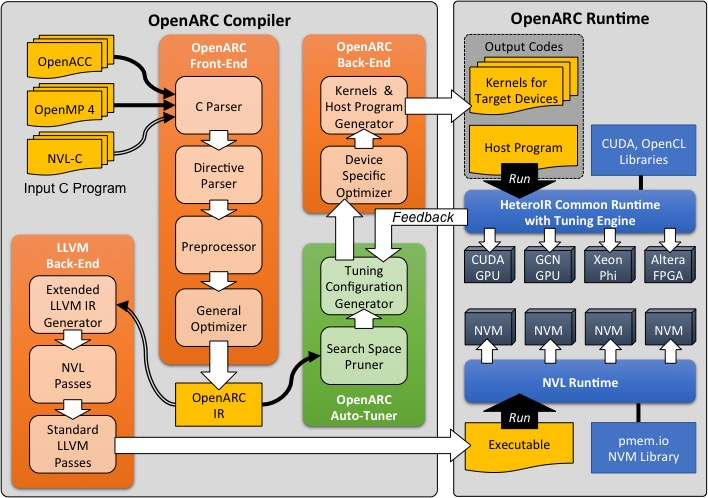
\includegraphics[width=6cm]{doc/perf_portability/openarc_all}
  \end{center}

  {\small source: \myurl{http://ft.ornl.gov/research/openarc}}

\end{frame}


\end{document}
